\documentclass[11pt]{article}

\usepackage[margin=1in]{geometry}
\usepackage[T1]{fontenc}
\usepackage{lmodern}
\usepackage{microtype}
\usepackage{amsmath,amssymb,amsthm,mathtools}
\usepackage[dvipsnames]{xcolor}
\usepackage[most]{tcolorbox}
\usepackage{tikz}
\usepackage{enumitem}
\usepackage{tocloft}
\usepackage[hidelinks]{hyperref}

\definecolor{courseblue}{HTML}{1F4E79}
\definecolor{lightblue}{HTML}{EAF2F8}
\definecolor{lightgreen}{HTML}{EAF7EA}
\definecolor{lightpink}{HTML}{FCE8EF}
\definecolor{lightyellow}{HTML}{FFF8D6}
\definecolor{warningyellow}{HTML}{D6A000}
\definecolor{darkgray}{HTML}{333333}

\setlength{\parindent}{0pt}
\setlength{\parskip}{0.65em}
\setlist[itemize]{topsep=0.25em,itemsep=0.15em}
\renewcommand{\cftsecleader}{\cftdotfill{\cftdotsep}}
\renewcommand{\cftsubsecleader}{\cftdotfill{\cftdotsep}}

\theoremstyle{plain}
\newtheorem{theorem}{Theorem}[section]
\newtheorem{proposition}[theorem]{Proposition}
\newtheorem{lemma}[theorem]{Lemma}
\newtheorem{corollary}[theorem]{Corollary}
\theoremstyle{definition}
\newtheorem{definition}[theorem]{Definition}
\newtheorem{example}[theorem]{Example}
\newtheorem{exercise}[theorem]{Exercise}
\theoremstyle{remark}
\newtheorem*{remark}{Remark}
\newtheorem*{fact}{Fact}
\newtheorem*{warning}{Warning}

\tcolorboxenvironment{definition}{
  enhanced,
  colback=lightgreen,
  colframe=ForestGreen,
  boxrule=0.7pt,
  arc=2pt,
  left=6pt,
  right=6pt,
  top=5pt,
  bottom=5pt
}

\tcolorboxenvironment{exercise}{
  enhanced,
  colback=lightpink,
  colframe=WildStrawberry,
  boxrule=0.7pt,
  arc=2pt,
  left=6pt,
  right=6pt,
  top=5pt,
  bottom=5pt
}

\tcolorboxenvironment{warning}{
  enhanced,
  colback=lightyellow,
  colframe=warningyellow,
  boxrule=0.7pt,
  arc=2pt,
  left=6pt,
  right=6pt,
  top=5pt,
  bottom=5pt
}

\numberwithin{equation}{section}

\newcommand{\be}{\begin{eqnarray}}
\newcommand{\ee}{\end{eqnarray}}
\newcommand{\C}{\mathbb{C}}
\newcommand{\R}{\mathbb{R}}
\newcommand{\N}{\mathbb{N}}

\DeclareMathOperator{\Hol}{\mathcal{H}\mathrm{ol}}
\DeclareMathOperator{\Real}{Re}
\DeclareMathOperator{\Imag}{Im}
\newcommand{\A}{\mathcal{A}}
\newcommand{\CT}{\C[[T]]}
\newcommand{\CLT}{\C((T))}
\tcbset{breakable}
\begin{document}

\begin{center}
  \colorbox{lightblue}{%
    \begin{minipage}{0.94\textwidth}
      \vspace{0.55em}
      \begin{tabular*}{\textwidth}{@{\extracolsep{\fill}}lr}
        {\color{courseblue}\bfseries\LARGE Lecture 6} &
        {\color{courseblue}\bfseries\LARGE MATH 411}\\[0.35em]
        \textbf{Fall 2026} & \textbf{Date: Sep 16, 2026}\\
        & \textbf{Instructor: Manish Patnaik}
      \end{tabular*}
      \vspace{0.45em}
    \end{minipage}}
\end{center}

\setcounter{tocdepth}{1}
\tableofcontents
\vspace{0.45em}

% Handwritten page 1.
\section{Where we are going: holomorphic versus analytic}
Let $U\subseteq\C$ be an open set. Two classes of functions on $U$ will
occupy us for the next several lectures.

\begin{center}
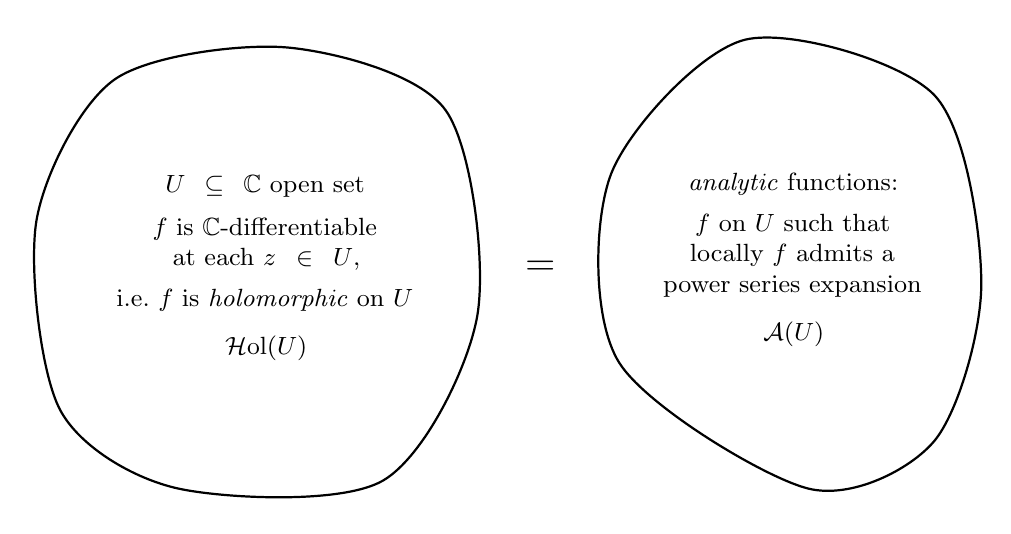
\begin{tikzpicture}[scale=1.0]
 \draw[thick] plot[smooth cycle] coordinates
  {(-6.1,-1.6) (-6.4,0.8) (-5.4,2.6) (-3.2,3.0) (-1.2,2.2) (-0.8,-0.4) (-2.0,-2.5) (-4.6,-2.6)};
 \node[align=center,text width=4.7cm,font=\small] at (-3.5,0.2)
  {$U\subseteq\C$ open set\\[0.5em]
   $f$ is $\C$-differentiable\\ at each $z\in U$,\\[0.4em]
   i.e.\ $f$ is \emph{holomorphic} on $U$\\[0.7em]
   $\Hol(U)$};
 \node[font=\Large] at (0.0,0.2) {$=$};
 \draw[thick] plot[smooth cycle] coordinates
  {(3.4,-2.6) (1.0,-1.0) (0.9,1.4) (2.6,3.1) (5.0,2.4) (5.6,0.0) (5.0,-2.0)};
 \node[align=center,text width=4.0cm,font=\small] at (3.2,0.3)
  {\emph{analytic} functions:\\[0.4em] $f$ on $U$ such that\\ locally $f$ admits a\\
   power series expansion\\[0.7em] $\A(U)$};
\end{tikzpicture}
\end{center}

The main theorem of this part of the course is that these two classes
coincide: $\Hol(U)=\A(U)$.

\begin{fact}[``proved'' last time using Green's theorem]
Let $\gamma\colon[a,b]\to U$ be a piecewise smooth, simple closed curve whose
interior lies in $U$, and let $f\in\Hol(U)$. Then
\be
 \int_\gamma f=0,
 \qquad\text{where}\qquad
 \int_\gamma f:=\int_a^b f(\gamma(t))\,\gamma'(t)\,dt.
\ee
\end{fact}

\begin{center}
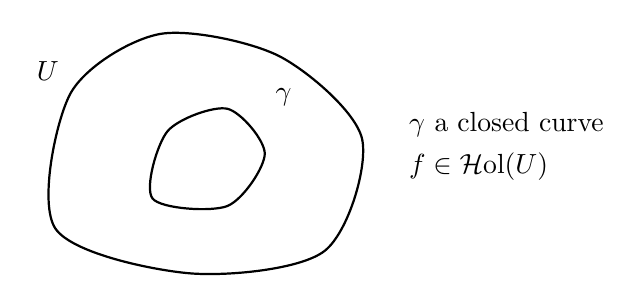
\begin{tikzpicture}[scale=0.95]
 \draw[thick] plot[smooth cycle] coordinates
  {(-2.2,-0.9) (-2.0,0.9) (-0.8,1.7) (0.8,1.4) (1.9,0.3) (1.4,-1.2) (-0.4,-1.5)};
 \draw[thick] plot[smooth cycle] coordinates
  {(-0.9,-0.5) (-0.7,0.4) (0.1,0.7) (0.6,0.1) (0.1,-0.6)};
 \node at (0.85,0.85) {$\gamma$};
 \node at (-2.3,1.2) {$U$};
 \node[right,align=left] at (2.4,0.2) {$\gamma$ a closed curve\\[0.3em] $f\in\Hol(U)$};
\end{tikzpicture}
\end{center}

We will prove this for \emph{analytic} functions directly (i.e.\ with no
Green's theorem), and then, once we know $\A(U)=\Hol(U)$, it will also hold
for $\Hol(U)$. The next few lectures therefore develop the machinery of
power series.

% Handwritten page 2.
\section{Formal power series}
Let $T$ be a \emph{formal variable}.

\begin{definition}
$\CT$ denotes the set of all expressions of the form
\be
 \sum_{n\ge0}a_nT^n=a_0+a_1T+a_2T^2+a_3T^3+\cdots,
 \qquad a_n\in\C.
\ee
These are the \emph{formal power series} over $\C$. No convergence is
required: a formal power series is just the sequence $(a_0,a_1,a_2,\dots)$
of its coefficients, written suggestively.
\end{definition}

What can we do with $\CT$? Let
\be
 f=a_0+a_1T+a_2T^2+\cdots,
 \qquad
 g=b_0+b_1T+b_2T^2+\cdots.
\ee

\subsection*{Addition}
\be
 f+g=(a_0+b_0)+(a_1+b_1)T+(a_2+b_2)T^2+\cdots.
\ee

\subsection*{Multiplication}
Multiplying power series:
\begin{align*}
 f\cdot g
 &=\bigl(a_0+a_1T+a_2T^2+\cdots\bigr)\bigl(b_0+b_1T+b_2T^2+\cdots\bigr)\\
 &=a_0b_0+(a_1b_0+a_0b_1)T+(a_0b_2+a_1b_1+a_2b_0)T^2+\cdots
\end{align*}
% Handwritten page 3.
that is,
\be
 f\cdot g=\sum_{n\ge0}\Biggl(\ \sum_{\substack{j+k=n\\j,k\ge0}}a_jb_k\Biggr)T^n.
\ee
Note that each coefficient is a \emph{finite} sum, so this makes sense
without any convergence hypothesis.

\subsection{Inversion}
When does $f\in\CT$ have a multiplicative inverse? Equivalently, when can we
find $g\in\CT$ such that $f\cdot g=1$?

Take $f$ fixed and $f,g$ as before. We want
\be
 a_0b_0+(a_1b_0+a_0b_1)T+(a_0b_2+a_1b_1+a_2b_0)T^2+\cdots=1,
\ee
i.e.\ $a_0b_0=1$ and every higher coefficient vanishes. To solve the first
equation we need $a_0\ne0$.

So assume $a_0\ne0$, and solve for the $b_n$ recursively:
\begin{align*}
 a_0b_0&=1 &&\Longrightarrow\quad b_0=a_0^{-1},\\
 a_1b_0+a_0b_1&=0 &&\Longrightarrow\quad b_1=-a_0^{-1}(a_1b_0),\\
 a_0b_2+a_1b_1+a_2b_0&=0 &&\Longrightarrow\quad b_2=-a_0^{-1}(a_1b_1+a_2b_0),
\end{align*}
and in general, having solved for $b_0,\dots,b_{n-1}$,
\be
 b_n=-a_0^{-1}\sum_{j=1}^{n}a_jb_{n-j}.
\ee

% Handwritten page 4.
\begin{proposition}
A power series $f=a_0+a_1T+\cdots\in\CT$ has an inverse if and only if
$a_0\ne0$.
\end{proposition}

\begin{example}
$f(T)=T$ is not invertible in $\CT$: its constant term is $0$.
\end{example}

\begin{remark}
If we set
\be
 \CLT=\text{all Laurent series of the form }\sum_{n\ge n_0}a_nT^n
 \qquad(n_0\in\mathbb Z),
\ee
then $\CLT$ is a \emph{field}, and $T$ does have an inverse in $\CLT$,
namely $T^{-1}$.
\end{remark}

\begin{example}
Let $f=1-T$. Solving $(1-T)(b_0+b_1T+b_2T^2+\cdots)=1$ coefficient by
coefficient gives
\be
 b_0=1,\qquad b_1-b_0=0\ \Longrightarrow\ b_1=1,
 \qquad b_2-b_1=0\ \Longrightarrow\ b_2=1,\qquad\dots
\ee
% Handwritten page 5.
so the inverse $(1-T)^{-1}$ looks like
\be
 (1-T)^{-1}=1+T+T^2+T^3+\cdots.
\ee
\end{example}

\subsection{Composition}
A more complicated operation on power series is called \emph{composition}.
Given $f(T)$ and $g(T)$, define $(f\circ g)(T)$ as
\be
 (f\circ g)(T)=a_0+a_1g(T)+a_2g(T)^2+a_3g(T)^3+\cdots.
\ee
This may or may not exist.

\begin{example}
Let $f=1+T+T^2+\cdots$ and $g(T)=1$. Then
\be
 f\circ g=1+1+1+\cdots
\ee
does not exist: the constant coefficient is an infinite sum of $1$'s.
\end{example}

\begin{proposition}
Assume $g(T)$ has no constant term, i.e.\ $b_0=0$. Then $f\circ g$ exists as
a power series.
\end{proposition}

% Handwritten page 6.
\begin{proof}
The expression $\sum_{n\ge0}a_ng(T)^n$ must be re-expanded as a series in
$T$ with well-defined coefficients. Since $b_0=0$, the series $g(T)^n$ is
divisible by $T^n$. Hence only the terms with $n\le m$ contribute to the
coefficient of $T^m$, so that coefficient is a finite sum.
\end{proof}

\subsection{Factorization}
Finally we state, without proof, the following simple observation.

\begin{proposition}
Every $f(T)\in\CLT$, $f \neq 0$, can be written as
\be
 f(T)=c\cdot T^k\cdot u(T),
 \qquad c\in\C,\ c\ne0,\quad k\in\mathbb{Z},
\ee
where $u(T)=1+a_1T+a_2T^2+\cdots$ is a power series with constant term $1$
(hence invertible).
\end{proposition}

\section*{Next goal: assigning a radius to a power series}
We want to assign to each $f(T)\in\CT$ a radius $r\in[0,\infty]$ so that if
\be
 z\in D(0,r)=\{z\in\C:|z|<r\},
\ee
then the series $f(z)=\sum_{n\ge0}a_nz^n$ converges, while if $|z|>r$ it
diverges.

\begin{center}
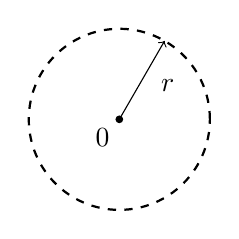
\begin{tikzpicture}[scale=1.0]
 \draw[thick,dashed] (0,0) circle (1.15);
 \fill (0,0) circle (1.4pt);
 \node[below left] at (0,0) {$0$};
 \draw[->] (0,0)--(60:1.15);
 \node at (35:0.75) {$r$};
\end{tikzpicture}
\end{center}

The extended nonnegative number $r$ is called the \emph{radius of
convergence} of $f$. To make sense of all this, we first need to recall
convergence in $\C$.

\begin{warning}
When $r<\infty$, we make no assertion about convergence on the circle
$|z|=r$; in fact, almost anything can happen there!
\end{warning}

% Handwritten page 7.
\section{Sequences and convergence}

We first review some standard notions concerning convergence of series,
phrased in the setting of complex numbers.


\begin{definition}
Let $\{z_n\}$ be a sequence of complex numbers.
\begin{enumerate}
\item We write
\be
 \boxed{\ w=\lim_{n\to\infty}z_n\ }
\ee
if, given any $\epsilon>0$, there exists $n_0$ such that if $n>n_0$ then
\be
 |w-z_n|<\epsilon.
\ee
\item We say that $\{z_n\}$ is a \emph{Cauchy sequence} if, given any
$\epsilon>0$, there exists $n_0$ such that if $m,n>n_0$ then
\be
 |z_m-z_n|<\epsilon.
\ee

\end{enumerate}
\end{definition}

\begin{remark}
Write $z_n=x_n+iy_n$. Then
\be
 |z_n-z_m|=\sqrt{(x_n-x_m)^2+(y_n-y_m)^2}.
\ee
Since $|x_n-x_m|\le|z_n-z_m|$ and $|y_n-y_m|\le|z_n-z_m|$, while
$|z_n-z_m|\le|x_n-x_m|+|y_n-y_m|$, we may use this to argue that
\be
 \{z_n\}\text{ Cauchy}
 \quad\Longleftrightarrow\quad
 \{x_n\}\text{ and }\{y_n\}\text{ are Cauchy sequences.}
\ee
\end{remark}

\begin{exercise}
Show that $\{z_n\}$ converges $\Longleftrightarrow$ $\{z_n\}$ is Cauchy.
(Use the same argument as in $\R$-analysis together with the remark above.)
\end{exercise}

Next, we turn to the notion of convergence of a series.


\begin{definition}
Let $a_n\in\C$.
\begin{enumerate}
\item $\displaystyle\sum_{n=0}^{\infty}a_n$ \emph{converges} if the sequence
$\{S_n\}$ of \emph{partial sums} converges, where
\be
 S_0=a_0,\quad S_1=a_0+a_1,\quad S_2=a_0+a_1+a_2,\quad\dots,\quad
 S_n=a_0+\cdots+a_n.
\ee
\item $\displaystyle\sum_{n=0}^{\infty}a_n$ is \emph{absolutely convergent}
if $\displaystyle\sum_{n=0}^{\infty}|a_n|$ is convergent.
\end{enumerate}
\end{definition}

Observe that, just as in real analysis, if $\sum a_n$ is absolutely
convergent, then it is convergent. Let
\be
 S_n:=\sum_{i=0}^n a_i
 \qquad\text{and}\qquad
 T_n:=\sum_{i=0}^n |a_i|.
\ee
Since $\sum |a_n|$ converges, the sequence $\{T_n\}$ is Cauchy. If $n>m$,
then
\be
 |S_n-S_m|
 =\left|\sum_{i=m+1}^n a_i\right|
 \leq\sum_{i=m+1}^n |a_i|
 =T_n-T_m
 =|T_n-T_m|.
\ee
Thus $\{S_n\}$ is Cauchy and therefore converges. Hence $\sum a_n$
converges.



\begin{theorem}[Comparison test]
\label{thm:comparison}
If $\sum c_n$ is a convergent series of nonnegative real numbers $c_n\ge0$,
and $\sum a_n$ is a series such that $|a_n|\le c_n$ for every $n\ge0$, then
$\sum a_n$ converges.
\end{theorem}

% Handwritten page 9.
\begin{proof}
The partial sums $\sum_{k=0}^{n}c_k$ are bounded above, since $\sum c_n$
converges. Moreover,
\be
 \sum_{k=0}^{n}|a_k|\le\sum_{k=0}^{n}c_k.
\ee
Thus the partial sums of $\sum_{n=0}^{\infty}|a_n|$ are bounded above.

From $\R$-analysis: if $\{b_n\}$ is a sequence of nonnegative numbers such
that the partial sums $t_k=\sum_{n=0}^{k}b_n$ are bounded above, then by the
least upper bound property\footnote{Every nonempty subset of $\R$ that is
bounded above has a least upper bound (supremum) in $\R$. More precisely, if
$S\subseteq\R$ is nonempty and bounded above, then there exists
$s=\sup S\in\R$ such that $x\le s$ for every $x\in S$, and for every
$\epsilon>0$ there exists $x\in S$ such that $s-\epsilon<x\le s$.} the
sequence $\{t_k\}$ converges because it is increasing and bounded above.
Applying this to $b_n=|a_n|$ shows $\sum|a_n|$ converges,
i.e.\ $\sum a_n$ converges absolutely, and hence converges.
\end{proof}

\section{Sequences of functions}
Let $S\subseteq\C$ be nonempty. For a bounded function $h:S\to\C$, define
its \emph{sup norm} by
\be
 \|h\|_S:=\sup_{z\in S}|h(z)|.
\ee

% Handwritten page 10.
\begin{definition}
Let $f_n,f:S\to\C$.
\begin{itemize}
\item We say $f_n$ \emph{converges pointwise} to $f$ if $f_n(z)\to f(z)$
for all $z\in S$.
\item We say $f_n$ \emph{converges uniformly} to $f$ if, given
$\epsilon>0$, there exists $n_0$ such that if $n\ge n_0$, then
\be
 |f_n(z)-f(z)|<\epsilon
 \qquad\text{for every }z\in S.
\ee
Equivalently, for every $\epsilon>0$, there exists $n_0$ such that
$\|f_n-f\|_S<\epsilon$ whenever $n\ge n_0$.
\end{itemize}
\end{definition}

\begin{definition}
The sequence $\{f_n\}$ is \emph{uniformly Cauchy} if, given $\epsilon>0$,
there is $n_0$ such that $|f_n(z)-f_m(z)|<\epsilon$ for every $z\in S$
whenever $m,n\ge n_0$. Equivalently, $\|f_n-f_m\|_S<\epsilon$.
\end{definition}

\begin{remark}
The difference between the two notions of convergence is the order of the
quantifiers: for pointwise convergence the index $n_0$ may depend on the
point $z\in S$, whereas for uniform convergence a single $n_0$ must work
for every $z\in S$ at once. We take this up next time.
\end{remark}

\end{document}
